\section{Experiment Analysis}
In this part, we will implement several unconstrained and constrained optimization alogorithms to solve minimum surfaces and obstacle problems respectively. More specificly, we will employ 3 basic unconstrained optimization algorithms (gradient descent method with backtracking, globalized Newton method, L- BFGS method) with 5 different boundary functions in the minimum surface problems. We will also consider how the discretization degree and addtional techniques influence our experimental results. For the obstacle problem, we will apply two constrained optimization algorithms (quadratic penalty method and projected gradient method) in combination with different obstacle functions. And meanwhile, we will analyze the perfomance of different implemented algorithms and discuss some potential improvements.
\subsection{Minimum Surfaces}
At first, we will illustrate five different boundary functions. Then we will choose one advanced algorithm to solve the minimum surface problem with five boundary functions and different discretization degree. Subsequently, we utilize other unconstrained optimization alogorithms and compare their perfomance from the perspective of relative objective function gap and iteration of norm of gradients. Finally, additional techniques such as exact line search, Barzilai-Borwein steps and inertial techniques will be introduced to accelerate the convergence process.
\subsubsection{Boundary Functions}
Here, figure \ref{fig:boundary} presents five different boundary function mentioned in the report requirement document. We will then determine the minimum surfaces using different boundary functions via our proposed algorithms.
\begin{figure}[!htbp]
    \centering
    \subfigure[$ r_1(x, y)=1+\sin (2 \pi x)$]
    {
    \centering
    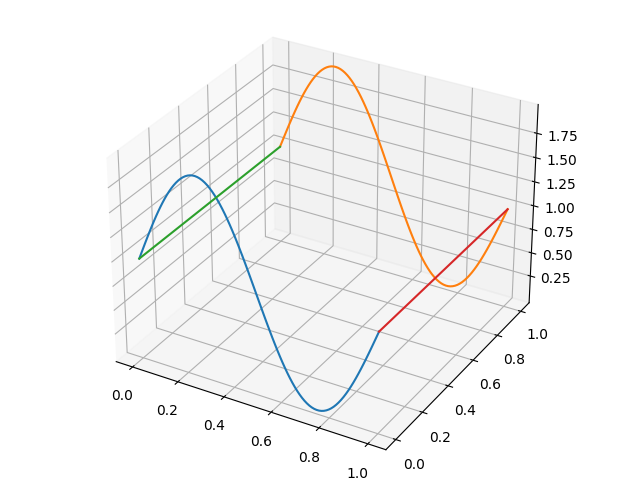
\includegraphics[width=0.3\columnwidth]{images/boundary/sin.png}
    }
    \subfigure[$ r_2(x, y)=1+\cos (1 / (x+0.001) )$]
    {
    \centering
    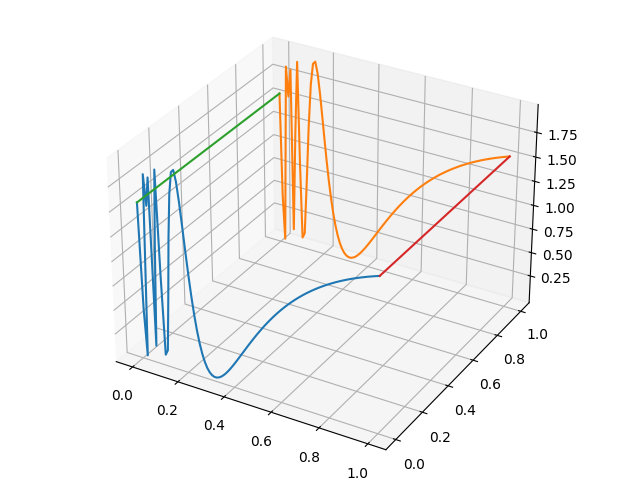
\includegraphics[width=0.3\columnwidth]{images/boundary/cos.png}
    }
    \subfigure[$ r_3(x, y)=\frac{1}{2}-\left|y-\frac{1}{2}\right|$]
    {
    \centering
    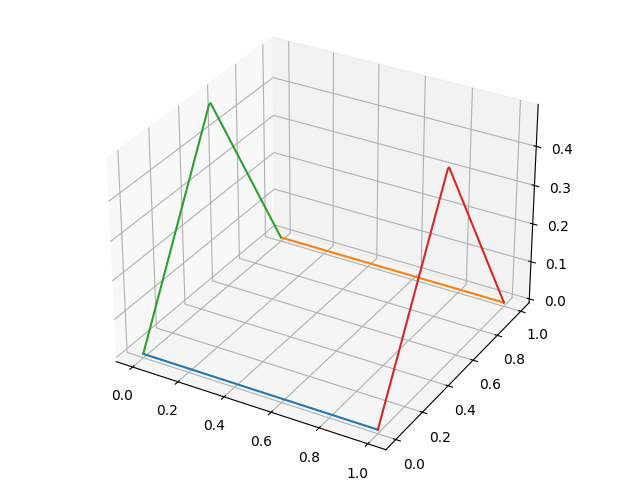
\includegraphics[width=0.3\columnwidth]{images/boundary/abs.png}
    }
    \subfigure[$ r_4(x, y)=(1+\exp (x y))^{-1}$]
    {
    \centering
    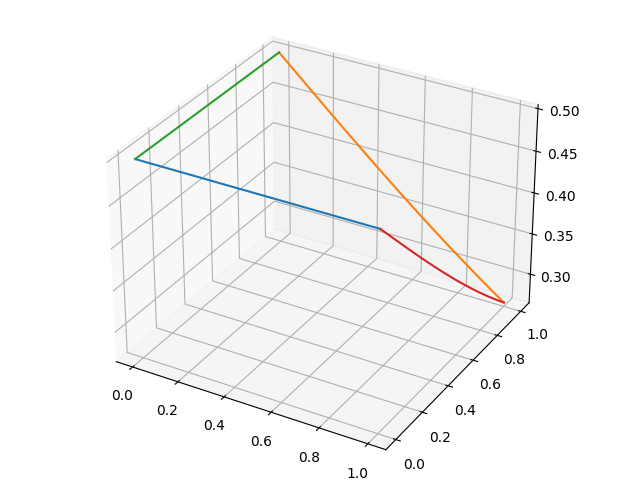
\includegraphics[width=0.3\columnwidth]{images/boundary/exp.png}
    }
    \subfigure[$ r_5(x, y)=1+\arcsin (-1+2 \sqrt{x y})$]
    {
    \centering
    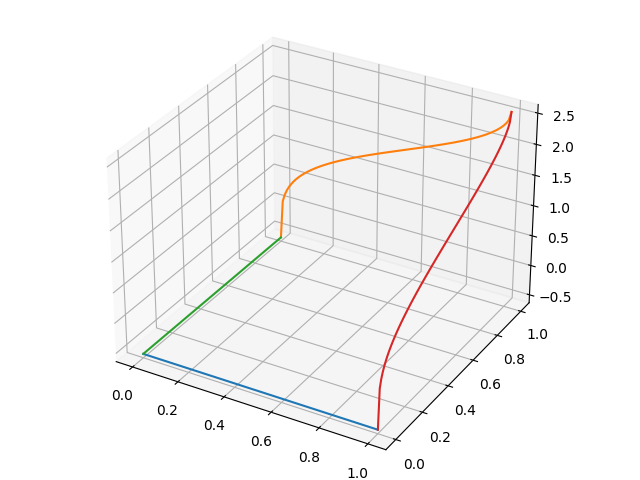
\includegraphics[width=0.3\columnwidth]{images/boundary/asin.png}
    }
    \caption{Five Boundaries in the Minimal Surface Problem (n=100)}
    \label{fig:boundary}  
\end{figure}
\subsubsection{Minimum Surface Results}
In order to demonstrate how the boundary function and discretization degree influence the minimal surface area, we choose globalized newton method to test these effects.

Comparing the corresponding subfigures between figure \ref{fig:boundary} and figure \ref{fig:min_surf_boundaries}, we can intuitively find out how the minimum surface come into shape. In order to control convariate, we choose $n=9$ and then generate the minimum surfaces under different boundaries. 

The minimal surface area depends on the number of the grid points. Figure \ref{fig:min_surf_discretization} shows how the discretization degree affect the formulation of minimum surface. It can be seen that the minimum surface becomes more and more smooth with larger discretization degree. As represented in table \ref{tab:per_vs_dis}, with the increase of the number of grid points, the minimal area is decreasing on the whole. With reference to the principle of calculus, we know the approximate error will be reduced with more grid points.In addition, with the increase of the number of discretization degree, the number of the variable is increasing, so the computation becomes slower and the iteration number also increases. 



\begin{table}[!ht]
    \caption{Perfomance Analysis with Different Discretization Degree}\label{tab:per_vs_dis}
    \begin{tabular*}{\hsize}{@{}@{\extracolsep{\fill}}cccc@{}}
    \toprule
             &Iteration number  &Final objective function  &Cost time(s)  \\
    \midrule
    $n=5$   &6   &2.4897  &0.371  \\
    $n=7$   &5   &2.4514  &0.752  \\
    $n=9$   &11  &2.4359  &2.855  \\
    $n=13$  &12  &2.4237  &7.152  \\
    $n=15$  &13  &2.4210  &10.868 \\
    $n=18$  &15  &2.4140  &18.741 \\
    \bottomrule
    \end{tabular*}
\end{table}

\begin{figure}[!htbp]
    \centering
    \subfigure[$ r_1(x, y)=1+\sin (2 \pi x)$]
    {
    \centering
    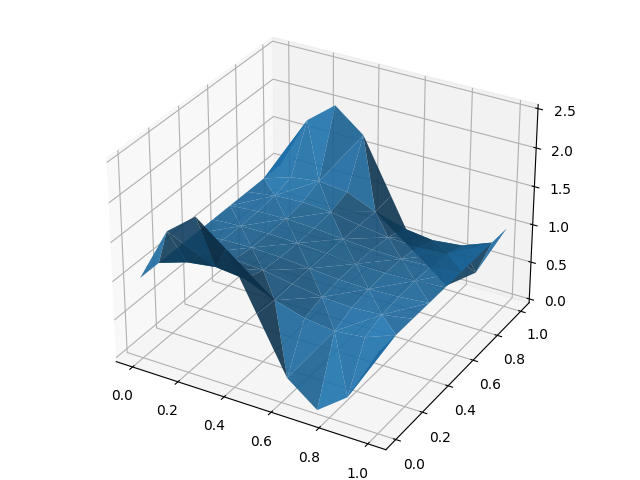
\includegraphics[width=0.3\columnwidth]{images/simple/min_surf_r0.png}
    }
    \subfigure[$ r_2(x, y)=1+\cos (1 / (x+0.001) )$]
    {
    \centering
    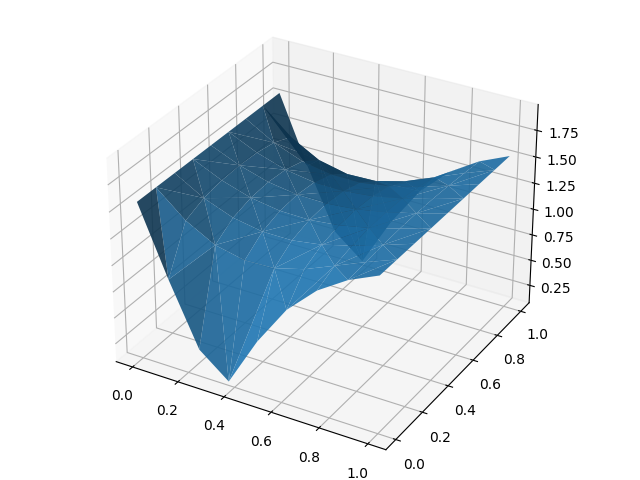
\includegraphics[width=0.3\columnwidth]{images/simple/min_surf_r1.png}
    }
    \subfigure[$ r_3(x, y)=\frac{1}{2}-\left|y-\frac{1}{2}\right|$]
    {
    \centering
    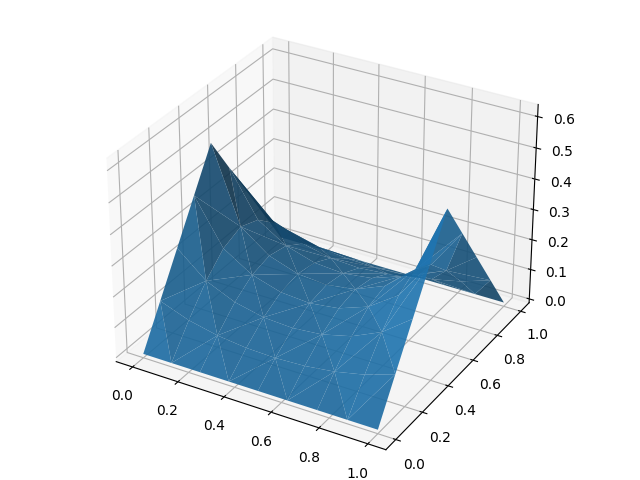
\includegraphics[width=0.3\columnwidth]{images/simple/min_surf_r2.png}
    }
    \subfigure[$ r_4(x, y)=(1+\exp (x y))^{-1}$]
    {
    \centering
    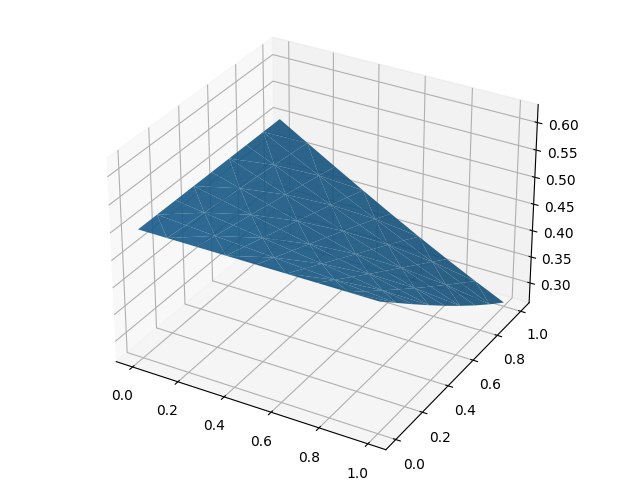
\includegraphics[width=0.3\columnwidth]{images/simple/min_surf_r3.png}
    }
    \subfigure[$ r_5(x, y)=1+\arcsin (-1+2 \sqrt{x y})$]
    {
    \centering
    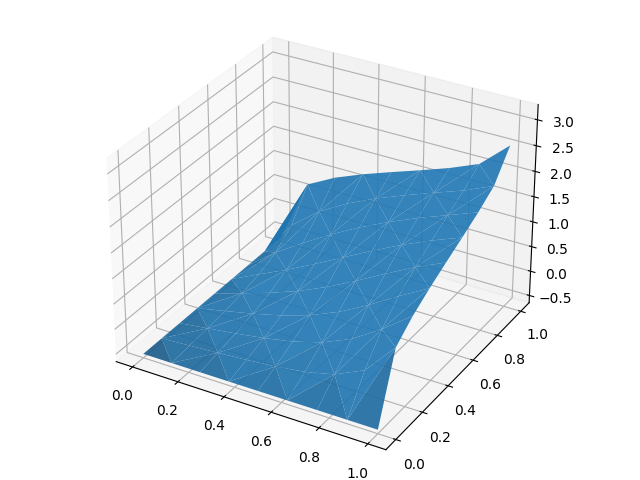
\includegraphics[width=0.3\columnwidth]{images/simple/min_surf_r4.png}
    }
    \caption{Minimum Surface Results with Five boundaries ($n=9$)}
    \label{fig:min_surf_boundaries}  
\end{figure}

\begin{figure}[!htbp]
    \centering
    \subfigure[$ r_2(x, y)$ with $n=5$]
    {
    \centering
    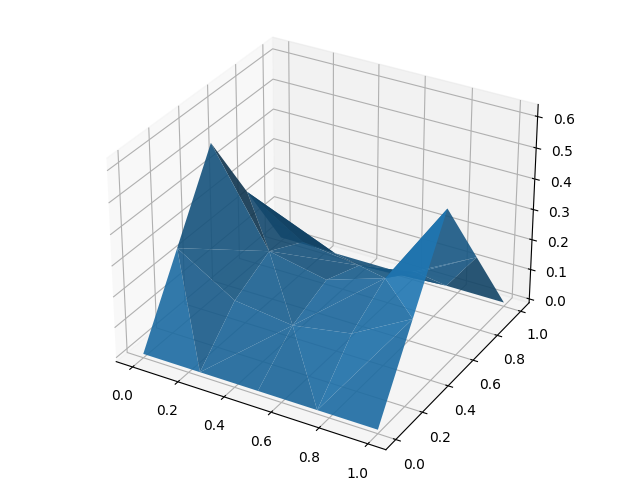
\includegraphics[width=0.3\columnwidth]{images/simple/min_surf_n5.png}
    }
    \subfigure[$ r_2(x, y)$ with $n=7$]
    {
    \centering
    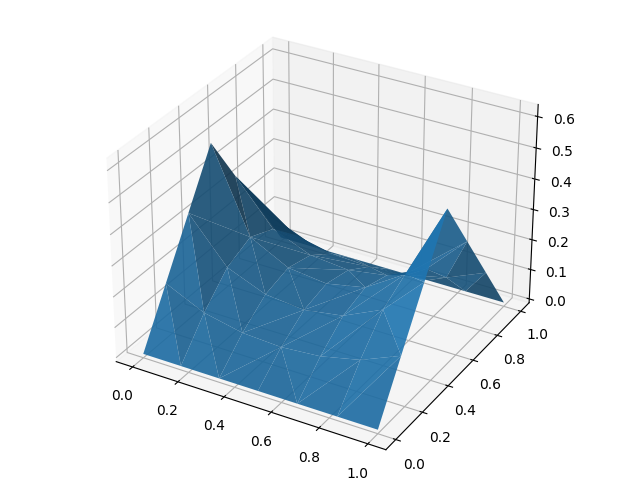
\includegraphics[width=0.3\columnwidth]{images/simple/min_surf_n7.png}
    }
    \subfigure[$ r_2(x, y)$ with $n=9$]
    {
    \centering
    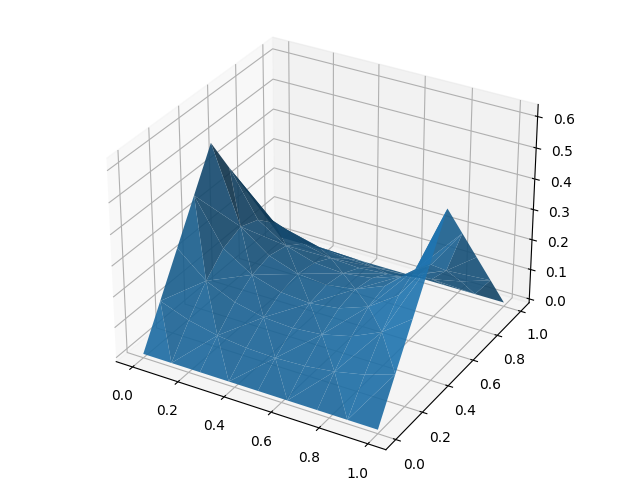
\includegraphics[width=0.3\columnwidth]{images/simple/min_surf_n9.png}
    }
    \subfigure[$ r_2(x, y)$ with $n=13$]
    {
    \centering
    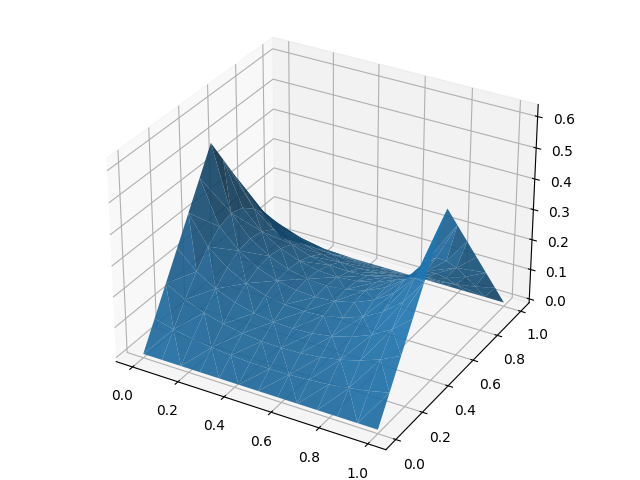
\includegraphics[width=0.3\columnwidth]{images/simple/min_surf_n13.png}
    }
    \subfigure[$ r_2(x, y)$ with $n=15$]
    {
    \centering
    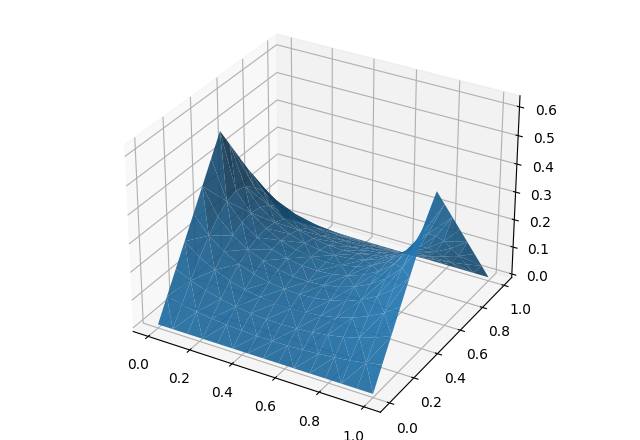
\includegraphics[width=0.3\columnwidth]{images/simple/min_surf_n15.png}
    }
    \subfigure[$ r_2(x, y)$ with $n=18$]
    {
    \centering
    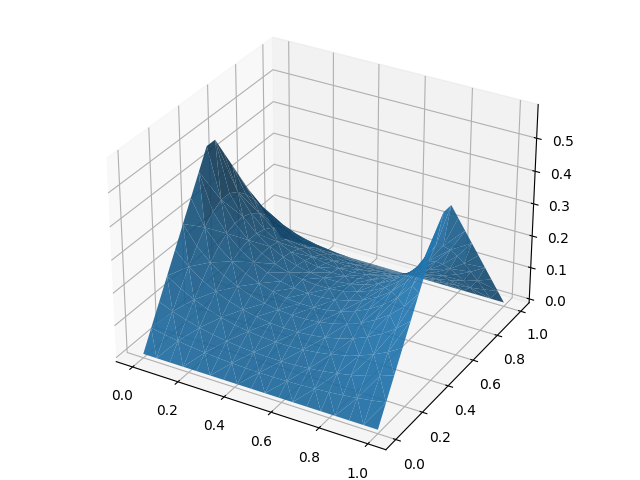
\includegraphics[width=0.3\columnwidth]{images/simple/min_surf_n18.png}
    }
    \caption{Minimum surface results with different discretization degree}
    \label{fig:min_surf_discretization}  
\end{figure}
\subsubsection{Perfomance Analysis}

In this section, we will compare the performance of the basic gradient descent method with backtracking, globalized newton method and the L-BFGS method. As we will introduce the overall performance comparison in next section, we mainly focus on the experimental results of these alogorithms via considering different discretization degree. Here, we set the boundary function $r(x, y)=\frac{1}{2}-\left|y-\frac{1}{2}\right|$. As illustrated in figure \ref{fig:alg_performance}, we can similarly conclude that the surface area becomes more smooth with larger $n$.
\begin{figure}[!htbp]
    \centering
    \subfigure[Gradient method with $n=7$]
    {
    \centering
    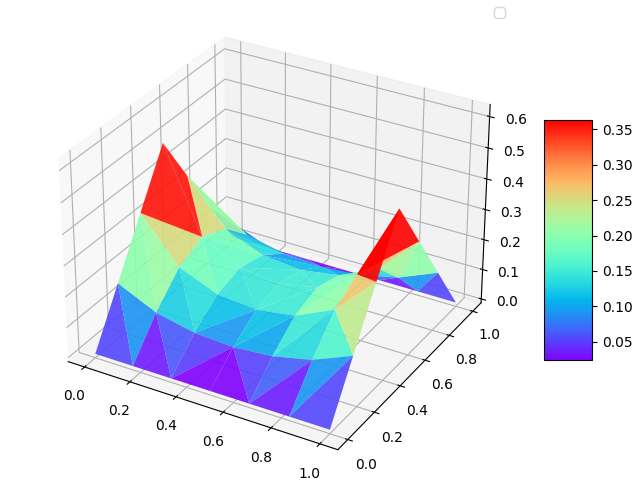
\includegraphics[width=0.3\columnwidth]{images/n_7_r_abs_ini_2/Gradient_Armijo.png}
    }
    \subfigure[Globalized newton method with $n=7$]
    {
    \centering
    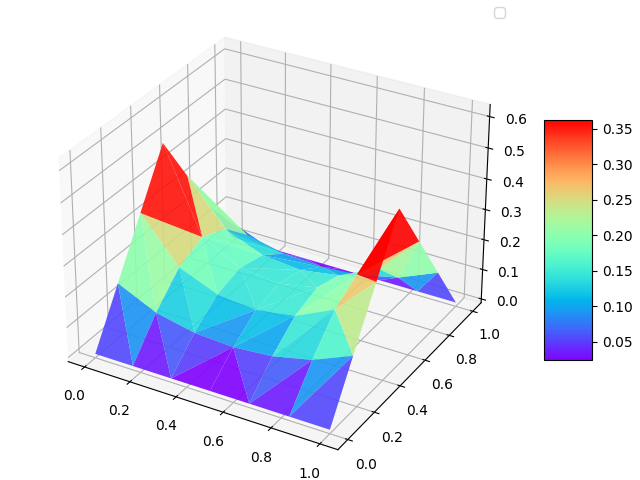
\includegraphics[width=0.3\columnwidth]{images/n_7_r_abs_ini_2/Globalized_Newton.png}
    }
    \subfigure[L-BFGS method with $n=7$]
    {
    \centering
    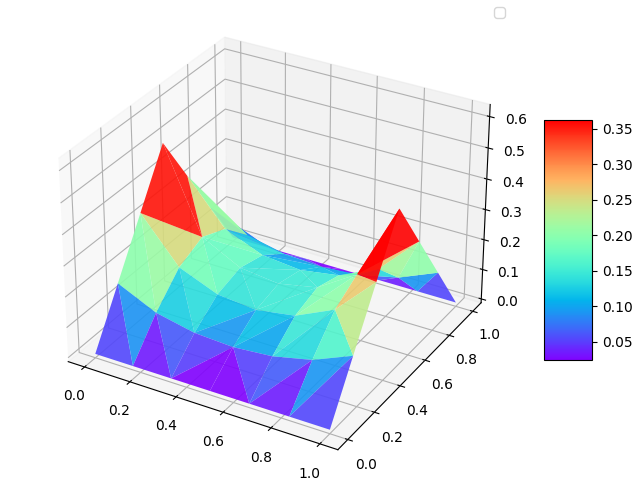
\includegraphics[width=0.3\columnwidth]{images/n_7_r_abs_ini_2/L-BFGS.png}
    }
    \subfigure[Gradient method with $n=17$]
    {
    \centering
    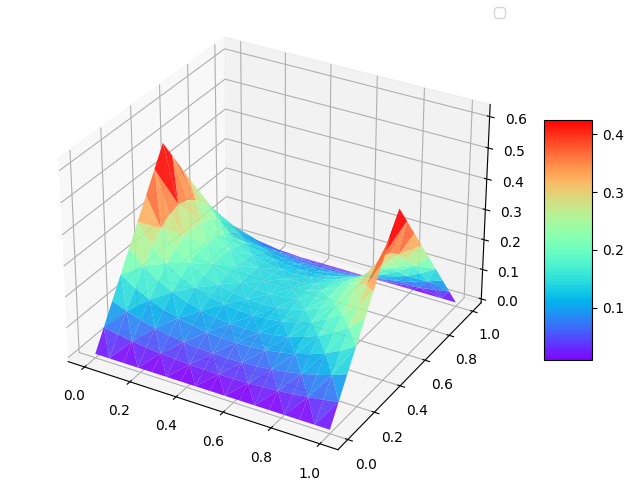
\includegraphics[width=0.3\columnwidth]{images/n_17_r_abs_ini_2/Gradient_Armijo.png}
    }
    \subfigure[Globalized newton method with $n$=17]
    {
    \centering
    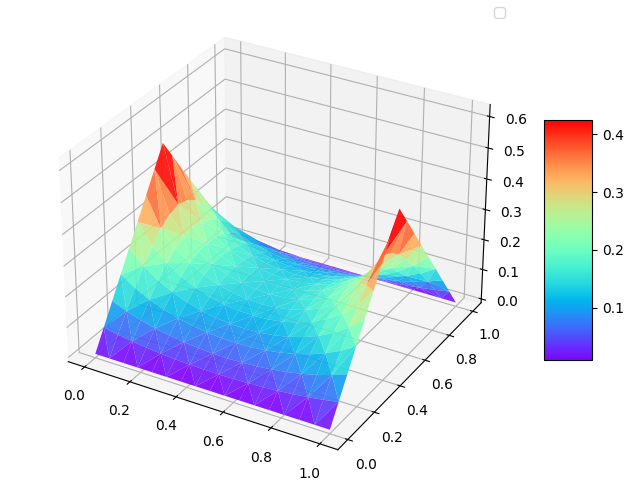
\includegraphics[width=0.3\columnwidth]{images/n_17_r_abs_ini_2/Globalized_Newton.png}
    }
    \subfigure[L-BFGS method with $n=17$]
    {
    \centering
    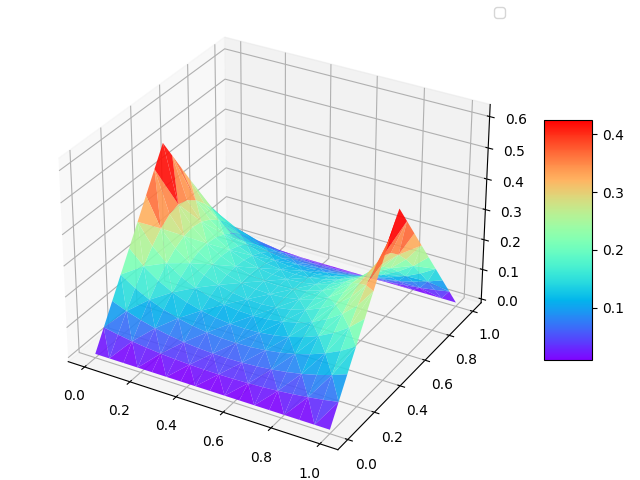
\includegraphics[width=0.3\columnwidth]{images/n_17_r_abs_ini_2/L-BFGS.png}
    }
    \caption{Minimum surface results via different algorithms with different discretization degree}
    \label{fig:alg_performance}  
\end{figure}
In table \ref{tab:per_n7} and table \ref{tab:per_n17}, we can intuitively conclude that globalized newton method perform best with the smallest iteration number and operation time while gradient method with backtracking shows the poorest performance, even though their final obejective values are very close.
\begin{table}[!ht]
    \caption{Perfomance Comparison under $n=7$}\label{tab:per_n7}
    \begin{tabular*}{\hsize}{@{}@{\extracolsep{\fill}}cccc@{}}
    \toprule
            &Iteration number  &Final objective function  &Cost time(s)  \\
    \midrule
    Gradient method   &77   &2.4514  &0.264  \\
    Globalized newton method   &5   &2.4514  &0.022  \\
    L-BFGS method   &19  &2.4514  &0.076  \\
    \bottomrule
    \end{tabular*}
\end{table}
\begin{table}[!ht]
    \caption{Perfomance Comparison under $n=17$}\label{tab:per_n17}
    \begin{tabular*}{\hsize}{@{}@{\extracolsep{\fill}}cccc@{}}
    \toprule
            &Iteration number  &Final objective function  &Cost time(s)  \\
    \midrule
    Gradient method   &780   &2.4191  &15.468  \\
    Globalized newton method   &13   &2.4194  &0.463  \\
    L-BFGS method   &46  &2.4191  &1.06  \\
    \bottomrule
    \end{tabular*}
\end{table}

\subsubsection{Additional Techniques}
In this part, we consider two more addtional techniques (exact line search and Barzilai-Borwein steps) to make comparison by the following two evalution metrics. One of the performance measures is to compare the relative objective function gap $\left|f\left(X^{k}\right)-f^{*}\right| / \max \left\{1,\left|f^{*}\right|\right\}$ with respect to the number of iterations and elapsed cpu-time. (Here $f^{*}$ denotes the optimal objective value obtained by each algorithm). Another evaluation is to compare the norm of gradients $\left(\left\|\Delta f\left(X^{k}\right)\right\|_{k}\right)$ with respect to the number of iterations and elapsed cpu-time.

In this case, we still set $r(x, y)=\frac{1}{2}-\left|y-\frac{1}{2}\right|$. When $n=17$, we can similarly get the minimum surface by the mentioned two additional techniques, as showned in figure \ref{fig:add_performance}.
\begin{figure}[!htbp]
    \centering
    \subfigure[Exact line search with $n=17$]
    {
    \centering
    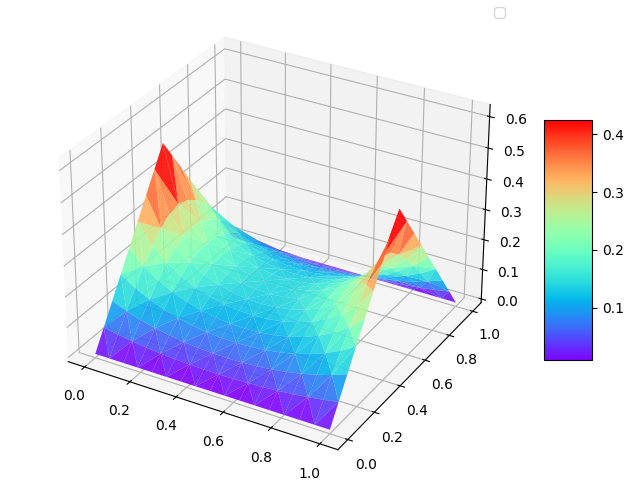
\includegraphics[width=0.42\columnwidth]{images/n_17_r_abs_ini_2/Exactline_Search.png}
    }
    \subfigure[Barzilai-Borwein steps with $n=17$]
    {
    \centering
    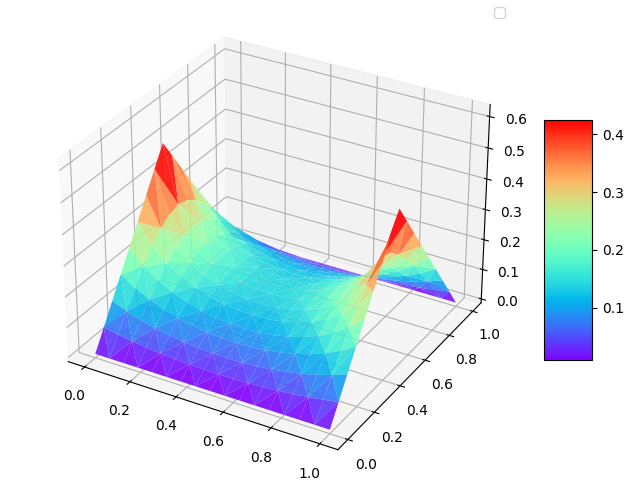
\includegraphics[width=0.42\columnwidth]{images/n_17_r_abs_ini_2/Barzilai_Borwein.png}
    }
    
    \caption{Minimum surface results via addtional techniques}
    \label{fig:add_performance}  
\end{figure}

Actually, the performance of these alogorithms vary according to our chosen performance measures. As presented in figure \ref{fig:performance_comparison}, we can demonstrate similarly that exact line search and gradient method with backtracking shows the poorer performance by analyzing the convergence curve. We can also derive a log-alogorithm to show the process of consective convergence. In figure \ref{fig:log_performance_comparison}, we can easily see the differences between different algorithms are magnified where globalized newton methods shows the best performance either from the perspective of relative objective function or norm of gradient.
\begin{figure}[!htbp]
    \centering
    \subfigure[Relative objective function gap vs number of iterations]
    {
    \centering
    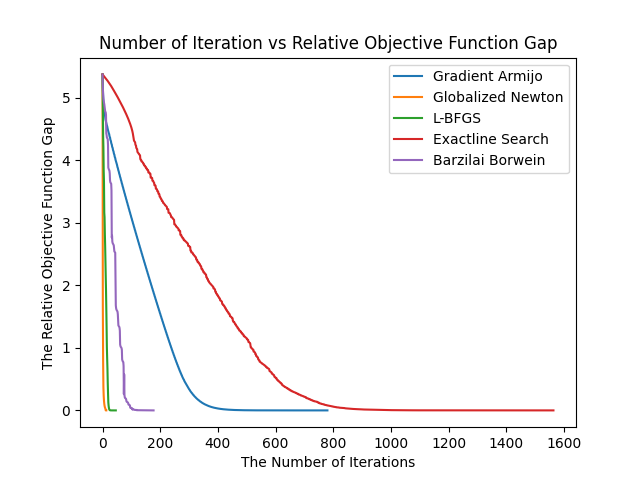
\includegraphics[width=0.42\columnwidth]{images/n_17_r_abs_ini_2/iter_gap.png}
    }
    \subfigure[Relative objective function Gap vs elapsed cpu-time]
    {
    \centering
    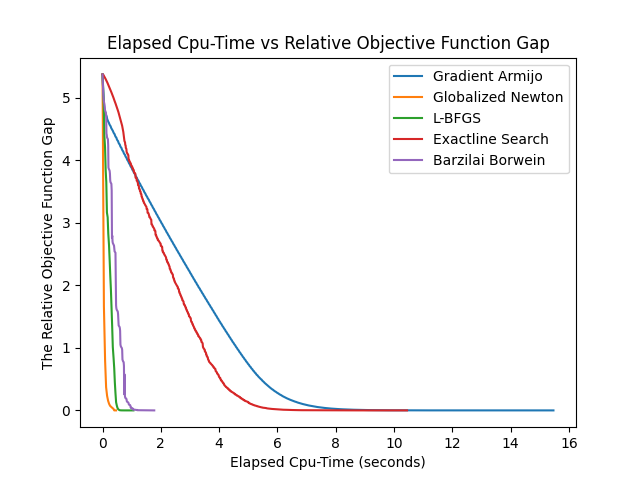
\includegraphics[width=0.42\columnwidth]{images/n_17_r_abs_ini_2/time_gap.png}
    }
    \subfigure[Norm of Gradients vs Number of Iterations]
    {
    \centering
    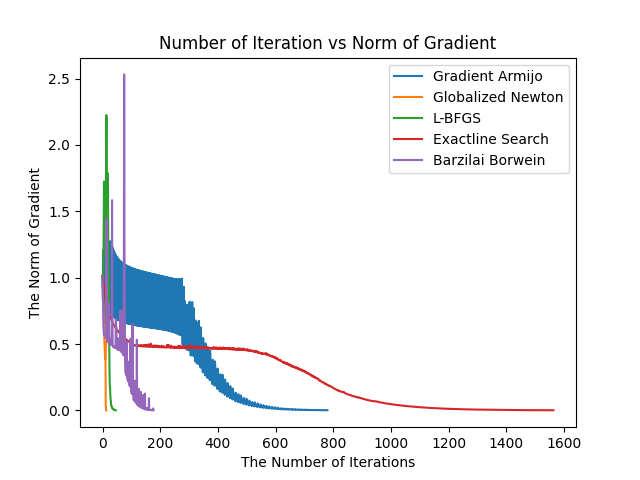
\includegraphics[width=0.42\columnwidth]{images/n_17_r_abs_ini_2/iter_g.png}
    }
    \subfigure[Norm of Gradients vs Number of Iterations]
    {
    \centering
    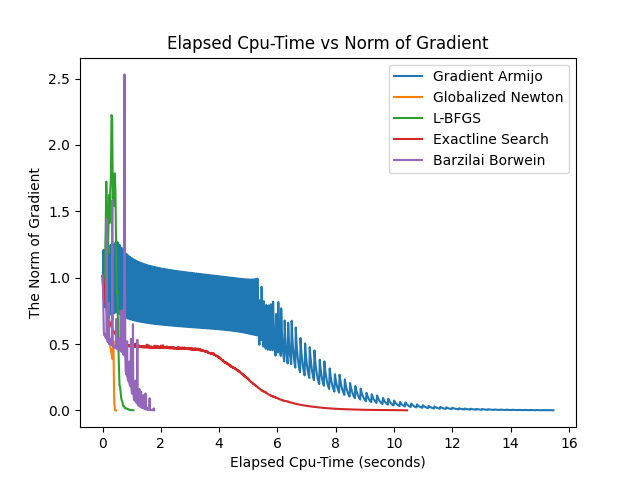
\includegraphics[width=0.42\columnwidth]{images/n_17_r_abs_ini_2/time_g.png}
    }
    \caption{Perfomance analysis via different algorithms}
    \label{fig:performance_comparison}  
\end{figure}

\begin{figure}[!htbp]
    \centering
    \subfigure[Logarithmic plot of relative objective function gap vs number of iterations]
    {
    \centering
    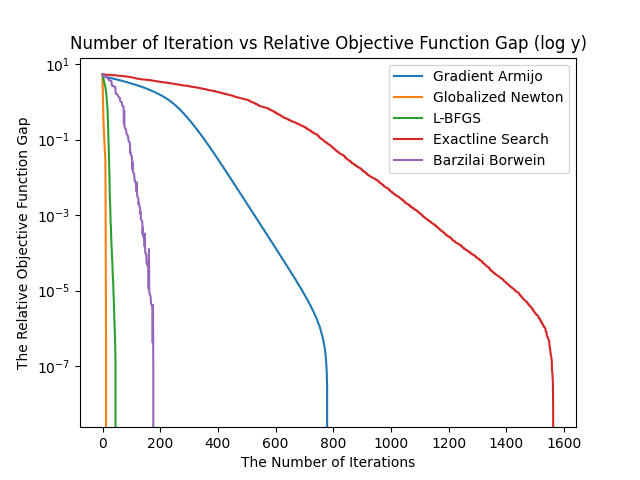
\includegraphics[width=0.42\columnwidth]{images/n_17_r_abs_ini_2/iter_gap_log_y.png}
    }
    \subfigure[Logarithmic plot of norm of gradients vs elapsed cpu-time]
    {
    \centering
    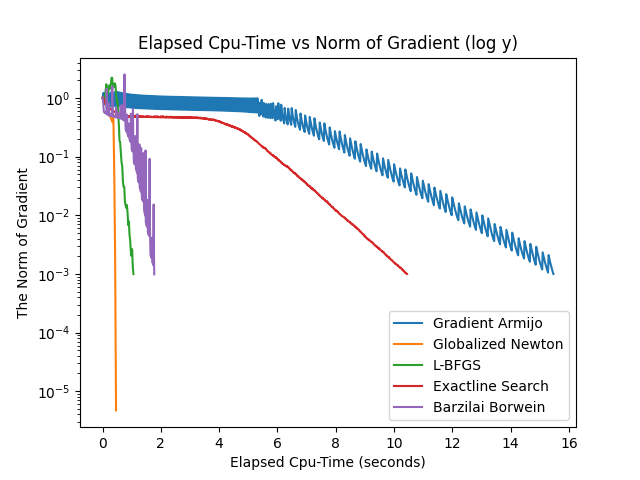
\includegraphics[width=0.42\columnwidth]{images/n_17_r_abs_ini_2/time_g_log_y.png}
    }
    \caption{Logarithmic plot of convergence performance}
    \label{fig:log_performance_comparison}  
\end{figure}
From the settings of our proposed experiments, intial points and maximum ietration number also play a vital part in the experimental results. Here, we set $n=7$ and iteration number as 20 or enough, and besides choose different intial points, to analyze how these factors influence our results. In figure \ref{fig:analysis_iteration}, it shows that exact line search method does not converge with limited iteration steps. As illustrated in figure \ref{fig:analysis_initial}, choosing different initial points can make the differences among these algorithms more obvious, where globalized newton methods still shows the best performance. 
\begin{figure}[!htbp]
    \centering
    \subfigure[Minimum surface: Exact line search with 20 iterations]
    {
    \centering
    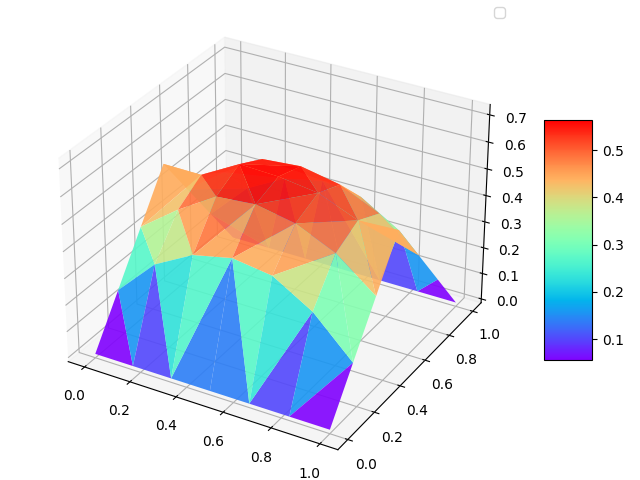
\includegraphics[width=0.45\columnwidth]{images/n_7_r_abs_ini_1/20_iter/Exactline_Search.png}
    }
    \subfigure[Minimum surface: Exact line search with enough iterations]
    {
    \centering
    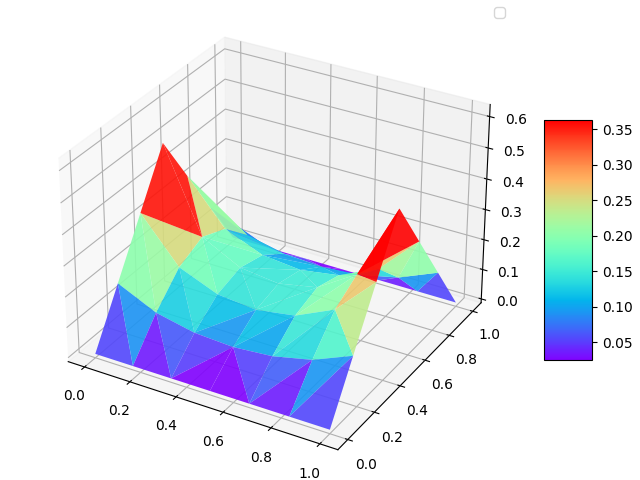
\includegraphics[width=0.45\columnwidth]{images/n_7_r_abs_ini_1/enough_iter/Exactline_Search.png}
    }
    \caption{Analysis of the influence of iteration setting}
    \label{fig:analysis_iteration}  
\end{figure}

\begin{figure}[!htbp]
    \centering
    \subfigure[Perfomance analysis with initial point 1]
    {
    \centering
    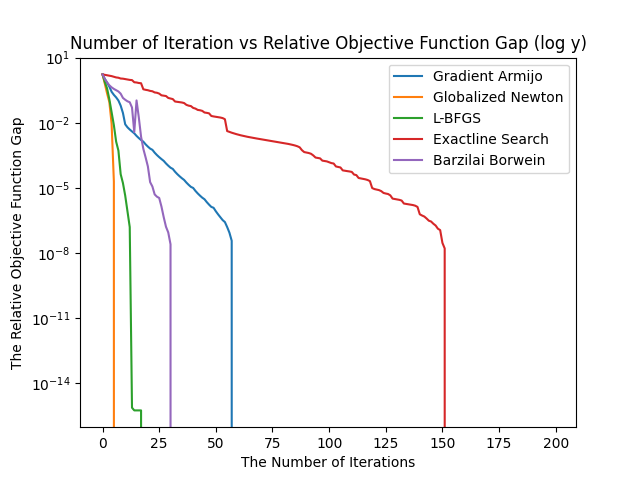
\includegraphics[width=0.42\columnwidth]{images/n_7_r_abs_ini_1/enough_iter/iter_gap_log_y.png}
    }
    \subfigure[Perfomance analysis with initial point 2]
    {
    \centering
    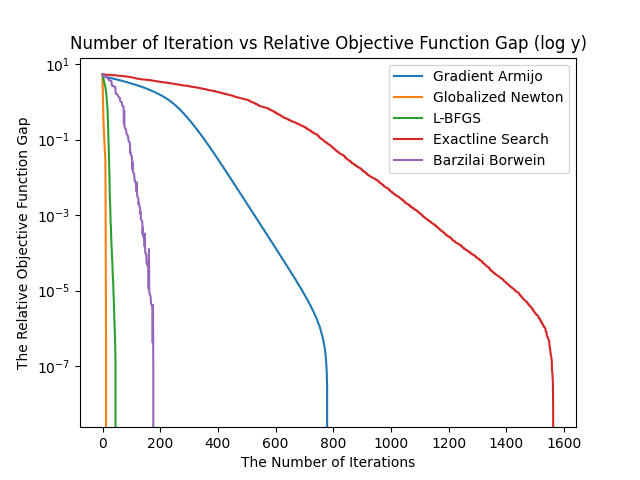
\includegraphics[width=0.42\columnwidth]{images/n_17_r_abs_ini_2/iter_gap_log_y.png}
    }
    \caption{Analysis of the influence of initial points}
    \label{fig:analysis_initial}  
\end{figure}


\subsection{Obstacle Problems}
As presented similarly in section 4.1, we firstly show different obstacles in the defiend boundary set via stochastic generation methods. We then choose projected gradient method to tackle the constrained optimization problem with different obstacle problems and illustrate corresponding minimum surface results. Lastly, We will equally present the perfomance camparing these two proposed algorithms. 
\subsubsection{Different Obstacles}
In our experiments, we generate the obstacles by designed and random methods. Figure \ref{fig:desined} shows our designed obstacles from different angle.

\begin{figure}[!htbp]
    \centering
    \subfigure[Designed generated obstacle]
    {
    \centering
    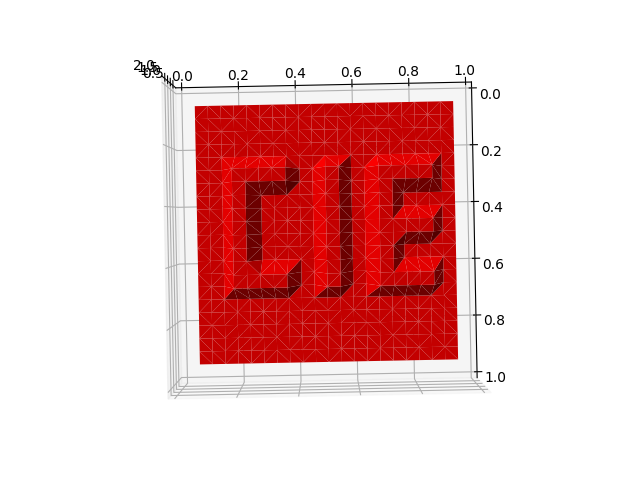
\includegraphics[width=0.42\columnwidth]{images/obstacle/origin/cie.png}
    }
    \subfigure[Designed generated obstacle]
    {
    \centering
    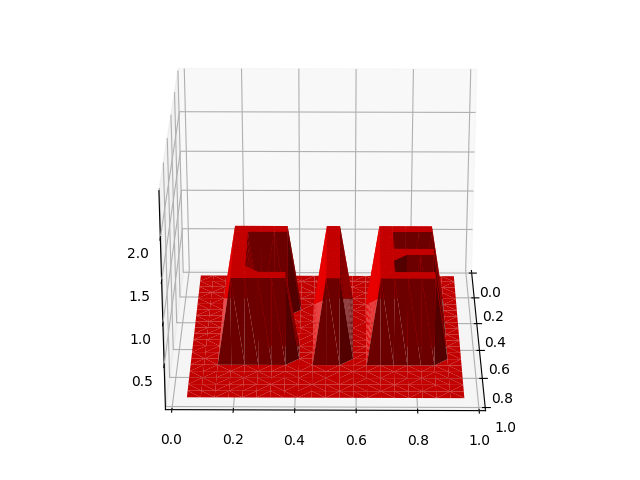
\includegraphics[width=0.42\columnwidth]{images/obstacle/origin/stochastic.png}
    }
    \caption{Illustration of designed generated obstacles}
    \label{fig:desined}  
\end{figure}

\subsubsection{Minimum Surface Results}
In this part, we will show our minimum surface results by implementing projected gradient method with five different boundary funtions. As presented in figure \ref{fig:min_des_obs} and figure \ref{fig:min_ran_obs}, we can vividly find out the process of generating minimum surfaces has been disturbed addtional obstacle constraints.
\begin{figure}[!htbp]
    \centering
    \subfigure[$ r_1(x, y)=1+\sin (2 \pi x)$]
    {
    \centering
    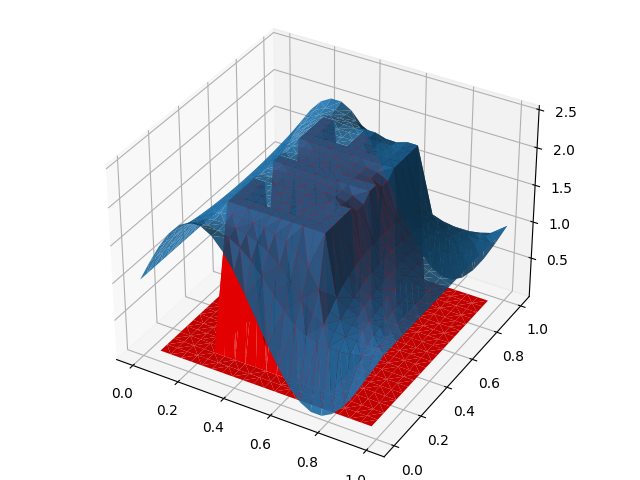
\includegraphics[width=0.3\columnwidth]{images/obstacle/cie/sin/sin_from_side.png}
    }
    \subfigure[$ r_2(x, y)=1+\cos (1 / (x+0.001) )$]
    {
    \centering
    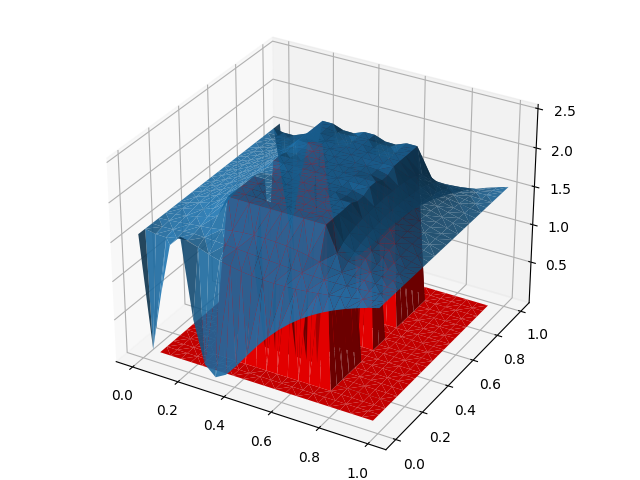
\includegraphics[width=0.3\columnwidth]{images/obstacle/cie/cos/cos_from_side.png}
    }
    \subfigure[$ r_3(x, y)=\frac{1}{2}-\left|y-\frac{1}{2}\right|$]
    {
    \centering
    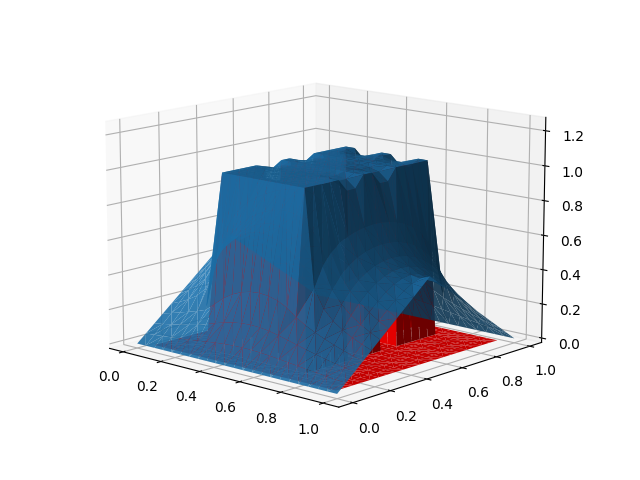
\includegraphics[width=0.3\columnwidth]{images/obstacle/cie/abs/abs_from_side.png}
    }
    \subfigure[$ r_4(x, y)=(1+\exp (x y))^{-1}$]
    {
    \centering
    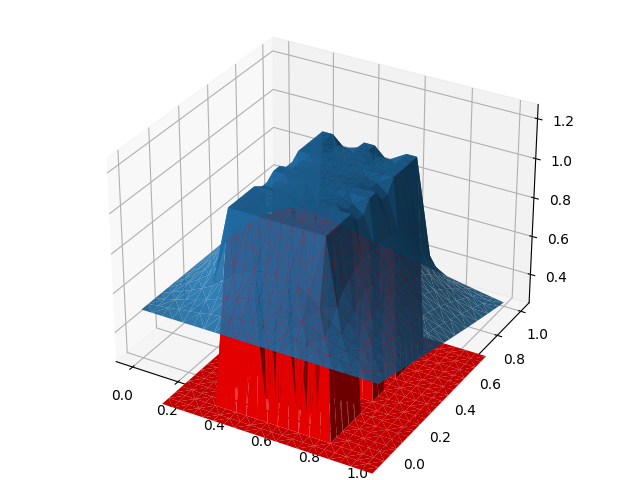
\includegraphics[width=0.3\columnwidth]{images/obstacle/cie/exp/exp_from_side.png}
    }
    \subfigure[$ r_5(x, y)=1+\arcsin (-1+2 \sqrt{x y})$]
    {
    \centering
    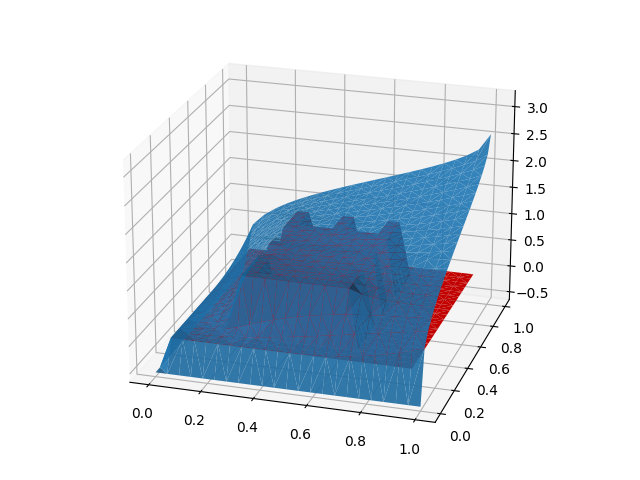
\includegraphics[width=0.3\columnwidth]{images/obstacle/cie/asin/asin_from_side.png}
    }
    \caption{Minimum Surface Results with Five Boundaries in Designed Obstacles}
    \label{fig:min_des_obs}  
\end{figure}
\begin{figure}[!htbp]
    \centering
    \subfigure[$ r_1(x, y)=1+\sin (2 \pi x)$]
    {
    \centering
    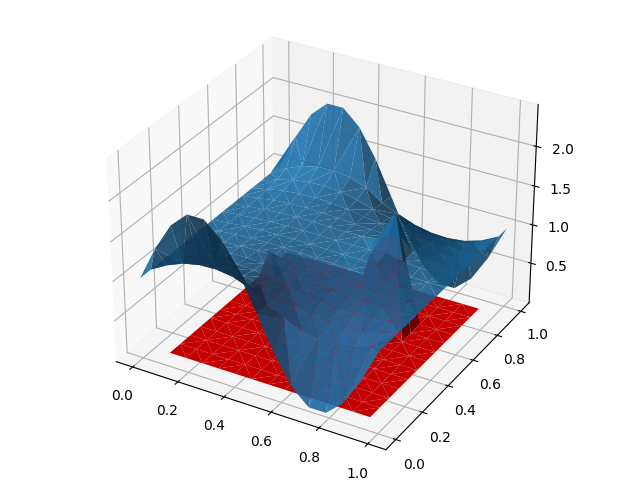
\includegraphics[width=0.3\columnwidth]{images/obstacle/random/sin/sin_from_side.png}
    }
    \subfigure[$ r_2(x, y)=1+\cos (1 / (x+0.001) )$]
    {
    \centering
    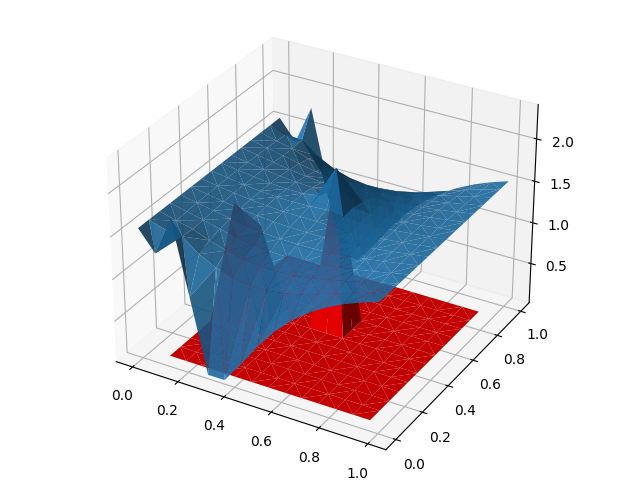
\includegraphics[width=0.3\columnwidth]{images/obstacle/random/cos/cos_from_side.png}
    }
    \subfigure[$ r_3(x, y)=\frac{1}{2}-\left|y-\frac{1}{2}\right|$]
    {
    \centering
    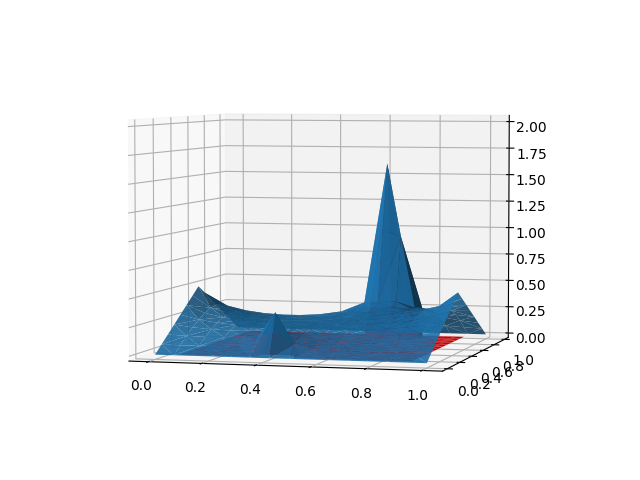
\includegraphics[width=0.3\columnwidth]{images/obstacle/random/abs/abs_from_side.png}
    }
    \subfigure[$ r_4(x, y)=(1+\exp (x y))^{-1}$]
    {
    \centering
    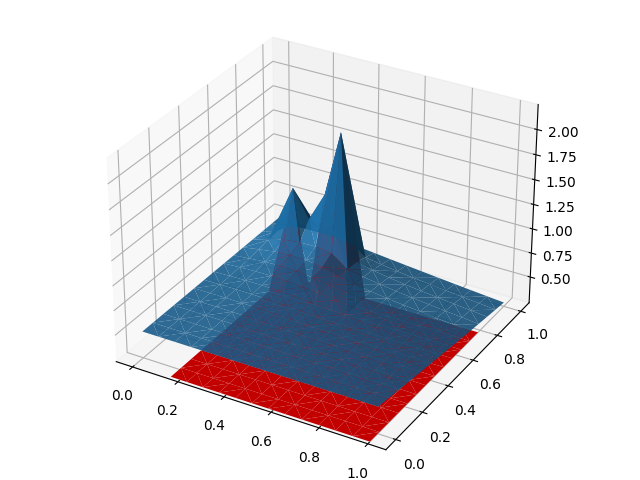
\includegraphics[width=0.3\columnwidth]{images/obstacle/random/exp/exp_from_side.png}
    }
    \subfigure[$ r_5(x, y)=1+\arcsin (-1+2 \sqrt{x y})$]
    {
    \centering
    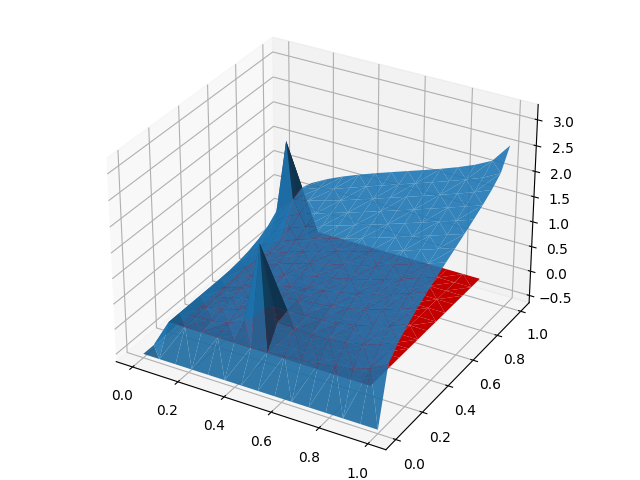
\includegraphics[width=0.3\columnwidth]{images/obstacle/random/asin/asin_from_side.png}
    }
    \caption{Minimum Surface Results with Five Boundaries in Random Obstacles}
    \label{fig:min_ran_obs}  
\end{figure}

\subsubsection{Perfomance Analysis}
Here we use the quadratic penalty method and the projected gradient armijo
method to solve the minimal surface problems with designed obstacles. Table \ref{tab:qua} shows one of the comparison results with the boundary funtion $ r_3(x, y)=\frac{1}{2}-\left|y-\frac{1}{2}\right|$. It can easily find that quadratic penalty method shows worse performance compared with projected gradient method with higher iteration number and operation time. This is because when implementing the penalty method, it needs a sub method to minimize the penalty function, which causes more iterations to converge and takes more operation time.
\begin{table}[!ht]
    \caption{Perfomance comparison between quadratic penalty method and projected gradient method}\label{tab:qua}
    \begin{tabular*}{\hsize}{@{}@{\extracolsep{\fill}}cccc@{}}
    \toprule
            &Iteration number  &Final objective function  &Cost time(s)  \\
    \midrule
    Projected gradient method    &784   &5.45  &19.18  \\
    Quadratic penalty method  &873   &5.45  &123.17  \\
    \bottomrule
    \end{tabular*}
\end{table}
